% Bottle Sumo Real-Time Streaming Firmware Report
% Generated by GitHub Copilot autonomous agent
\documentclass[11pt]{article}

\usepackage[a4paper,margin=1in]{geometry}
\usepackage{graphicx}
\usepackage{booktabs}
\usepackage{amsmath}
\usepackage{siunitx}
\usepackage{hyperref}
\usepackage{enumitem}
\usepackage{caption}
\usepackage{longtable}

\hypersetup{
  colorlinks=true,
  linkcolor=blue,
  urlcolor=cyan,
  pdfauthor={CTEA Bottle Sumo Project},
  pdftitle={Bottle Sumo RP2040 Firmware Architecture and Timing Report}
}

\setlist[itemize]{leftmargin=1.5em}
\setlist[description]{leftmargin=2.5em,labelindent=1em}

\title{Bottle Sumo Real-Time Streaming Firmware\\Architecture and Sensor Timing Report}
\author{CTEA Bottle Sumo Project}
\date{\today}

\begin{document}

\maketitle

\begin{abstract}
This report documents the dual-core firmware that powers the Bottle Sumo real-time streaming robot. It consolidates the execution responsibilities of Core~0 and Core~1, explains the shared-data synchronization strategy, and quantifies the timing budget for each sensor pipeline. The firmware reference for all observations is \texttt{BottleSumo\_RealTime\_Streaming.ino} (rev. \today).
\end{abstract}

\section{Firmware Overview}
The RP2040 application splits responsibilities across its two cores:
\begin{description}
  \item[Core~0 --- Control and Streaming] Initializes the I\textsuperscript{2}C bus, drives Wi-Fi access point and TCP telemetry (\S\ref{sec:streaming}), updates the OLED dashboard, and evaluates tactical decisions every \SI{10}{\milli\second} (\texttt{loop()}, lines~\texttt{933--1012}).
  \item[Core~1 --- Sensor Acquisition] Services the ADS1115-based QRE reflectance array and the VL53L0X distance sensors, publishing fresh samples into \texttt{SharedSensorData} via mutex-guarded writes (\texttt{loop1()}, lines~\texttt{1017--1041}).
\end{description}

The runtime shares measurement results and configuration through a trio of mutexes: \texttt{data\_mutex} protects sampled values, \texttt{wire1\_mutex} serializes OLED and ToF transactions on \texttt{Wire1}, and \texttt{threshold\_mutex} guards the adjustable edge-detection voltage (lines~\texttt{118--153}).

\section{Architecture Diagram}
Figure~\ref{fig:architecture} summarises the major execution blocks, buses, and data transfer paths. The diagram originates from the Mermaid source in \texttt{docs/bottle\_sumo\_architecture.mmd} and can be regenerated with the Mermaid CLI.

\begin{figure}[h]
  \centering
  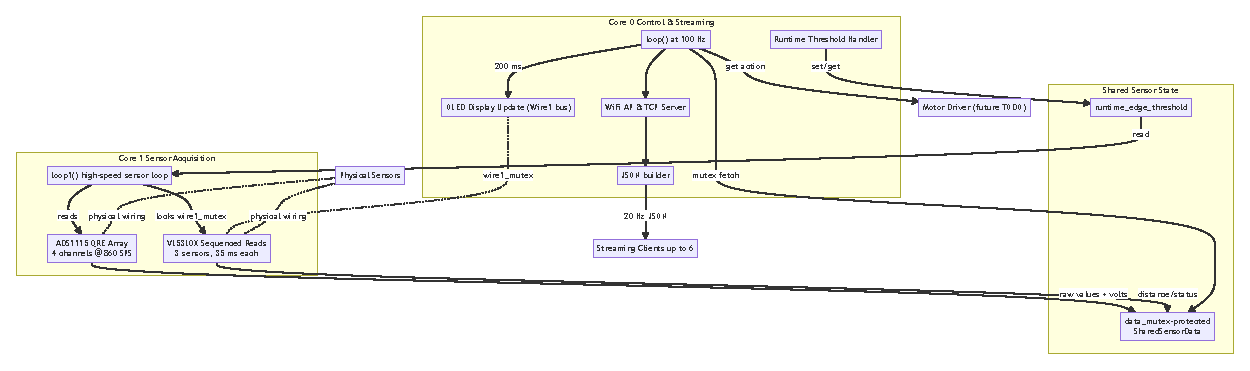
\includegraphics[width=0.95\linewidth]{bottle_sumo_architecture.pdf}
  \caption{High-level dual-core architecture and data flows.}
  \label{fig:architecture}
\end{figure}

\section{Sensor Pipelines and Timing}
The firmware budgets sensor time explicitly to guarantee that control and telemetry loops meet their deadlines. Table~\ref{tab:sensor-timing} aggregates configuration constants and measured latencies.

\begin{longtable}{@{}p{0.28\linewidth}p{0.18\linewidth}p{0.2\linewidth}p{0.26\linewidth}@{}}
\caption{Sensor timing budget}\label{tab:sensor-timing}\\
\toprule
Pipeline & Configuration Reference & Cycle Time & Notes \\
\midrule
\endfirsthead
\toprule
Pipeline & Configuration Reference & Cycle Time & Notes \\
\midrule
\endhead
\bottomrule
\endfoot
IR Reflectance (ADS1115) & \texttt{RATE\_ADS1115\_860SPS} (line~\texttt{520}) & \SI{1.16}{ms} per channel \newline \SI{4.6}{ms} for full burst & Four channels sampled sequentially inside \texttt{updateSharedIRData()} (lines~\texttt{1057--1078}); ADS conversion sets the throughput ceiling. \\
ToF Distance (VL53L0X x3) & \texttt{TOF\_TIMING\_BUDGET\_US = 35\,000} (lines~\texttt{37--44}) & \SI{35}{ms} per sensor \newline \SI{115}{ms} per sweep & Sensors are read sequentially under \texttt{wire1\_mutex} in \texttt{readToFSensors()} (lines~\texttt{601--676}); extra \SI{10}{ms} slack accounts for mutex and copy overhead. \\
Shared Data Publication & \texttt{TOF\_DATA\_FRESHNESS\_MS = 150} (line~\texttt{50}) & \SI{115}{ms} ToF freshness window \newline \SI{6}{ms} IR freshness window & \texttt{loop1()} pushes IR on every iteration and ToF when \texttt{now - lastToFUpdate \textgreater\, 115\,ms} (lines~\texttt{1020--1041}). \\
Control Loop (Core~0) & \texttt{delay(10)} (line~\texttt{1009}) & \SI{10}{ms} cadence & Each iteration validates data freshness, updates streaming clients, refreshes OLED every 50 iterations, and evaluates tactical state. \\
Telemetry Stream & \texttt{STREAM\_SEND\_INTERVAL = 50\,ms} (lines~\texttt{159--165}) & \SI{50}{ms} transmit cadence & JSON packets include core frequencies, IR thresholds, and ToF direction hints (lines~\texttt{861--912}). \\
\end{longtable}

The ToF cycle demonstrates the longest blocking section. Combining the constants yields Equation~\eqref{eq:tof-cycle}:
\begin{equation}
  t_{\text{ToF cycle}} = 3 \times \SI{35}{ms} + \SI{10}{ms} \approx \SI{115}{ms},
  \label{eq:tof-cycle}
\end{equation}
which aligns with the freshness tolerance enforced by \texttt{TOF\_DATA\_FRESHNESS\_MS}.

\section{Streaming and Telemetry}\label{sec:streaming}
Core~0 throttles TCP maintenance to \SI{40}{Hz} and emits telemetry at \SI{20}{Hz}. Each payload bundles IR voltages, ToF metrics, and inferred tactical state (\texttt{sendRealTimeStreamToAllClients()}, lines~\texttt{861--924}). The OLED dashboard is synchronized with the same shared data while respecting the I\textsuperscript{2}C mutex (\texttt{updateOLEDDisplay()}, lines~\texttt{680--759}).

\section{Verification Checklist}
\begin{itemize}
  \item Sensor acquisition split across cores; shared mutexes prevent I\textsuperscript{2}C contention.
  \item IR loop provides \SI{>150}{Hz} updates, matching the design banner displayed at boot (line~\texttt{707}).
  \item ToF loop maintains \SI{\leq115}{ms} age, satisfying \texttt{TOF\_DATA\_FRESHNESS\_MS} (line~\texttt{50}).
  \item Streaming cadence fixed at \SI{20}{Hz}, with Wi-Fi housekeeping decoupled to avoid blocking control logic.
\end{itemize}

\section{Reproduction Notes}
\begin{enumerate}
  \item Regenerate the Mermaid SVG/PDF: \texttt{mmdc -i docs/bottle\_sumo\_architecture.mmd -o docs/bottle\_sumo\_architecture.pdf}.
  \item Compile this report: \texttt{tectonic docs/bottle\_sumo\_report.tex} (or any LaTeX engine with \texttt{graphicx} and \texttt{siunitx}).
\end{enumerate}

\section{Appendix: Key Firmware Constants}
\begin{itemize}
  \item Wi-Fi AP configuration: lines~\texttt{72--105}.
  \item Streaming intervals and throttles: lines~\texttt{138--168}.
  \item Sensor data freshness thresholds: lines~\texttt{169--184}.
  \item Edge detection thresholds: lines~\texttt{190--207}.
\end{itemize}

\end{document}
